\section{Beobachter}

Bisher wurde von einer wesentlichen Vereinfachung der Realität ausgegangen. Nämlich dass für Stabilisierung, Zustandsrückführung \etc der gesamte Zustandsvektor des Kontrollsystems zur Verfügung steht. Tatsächlich sind in der Regel nicht alle Zustandsinformationen bekannt. Beispielsweise weil sie technisch überhaupt nicht messbar sind oder nur unter großem technischen beziehungsweise finanziellen Aufwand ermittelt werden könnten. Sprachlich wird
vereinfacht gesagt, dass die entsprechenden Größen \textit{nicht messbar} sind.

\begin{align*}
    dim(y) < dim(x)
\end{align*}

\begin{figure}[H]
    \centering
    \fbox{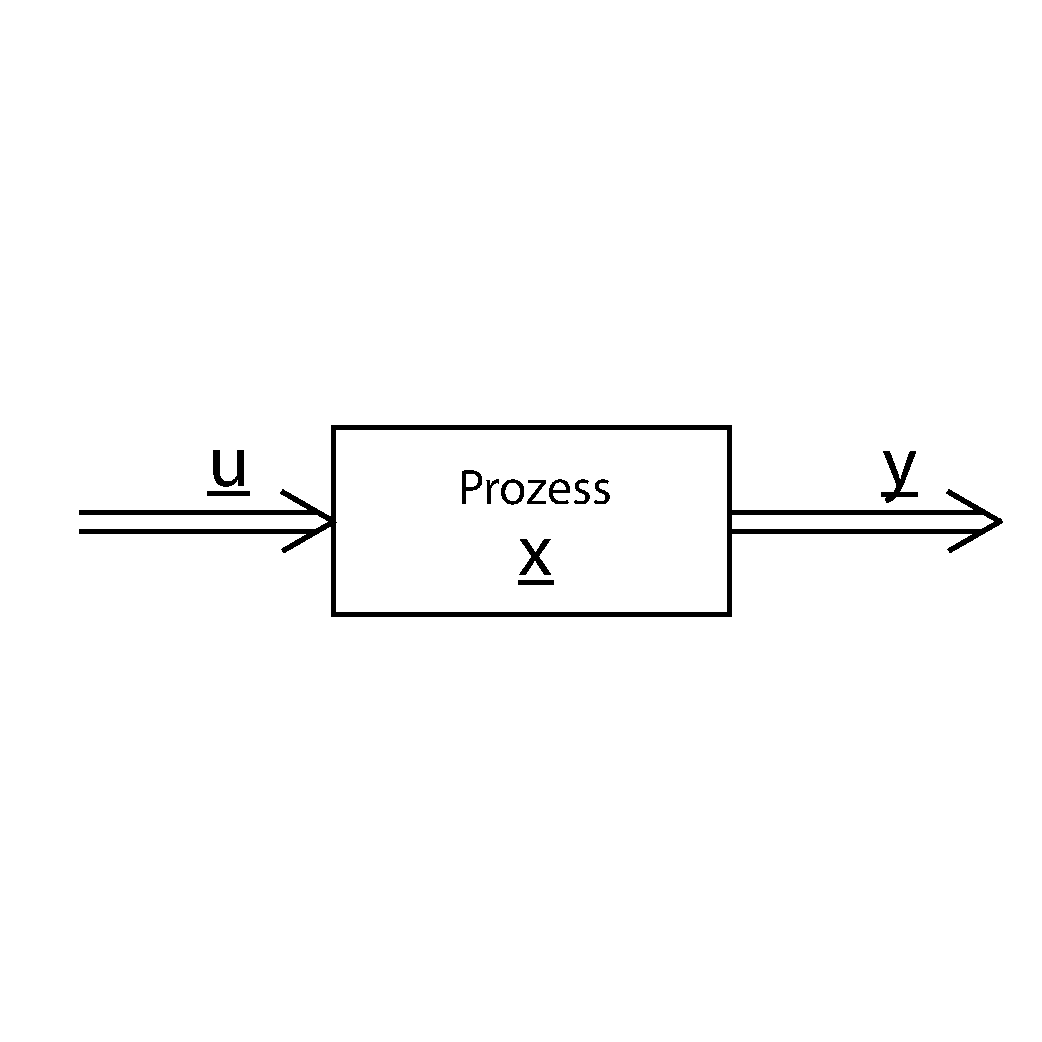
\includegraphics[width=0.5\textwidth]{Bilder/Beobachter/System.pdf}}
    \caption[Allgemeines System im Zustandsraum]{Schematische Darstellung eines allgemeinen Systems im Zustandsraum}
    \label{fig:Bild43}
\end{figure}

Da aber dennoch alle Zustände benötigt werden, da die Zustandsregelung darauf basiert, dass zu jedem Zeitpunkt alle Zustände bekannt sind, wird der Beobachter eingeführt.\\
Mit dessen Hilfe ist es möglich innere Zustände zu rekonstruieren. Dies erfolgt über ein \textbf{Modell} und dem \textbf{Vergleich} der rekonstruierten Zustände mit den gemessenen Ausgängen.\\
\newline
Ansatz von Luenberger:


\[
    \underline{\dot{\hat{x}}} = 
    \underbrace{% 
        A \cdot \underline{\hat{x}} + B \cdot \underline{u}
    }_{%
    Modell
    }
    + 
    \underbrace{%
    L \left( \underline{y} - \underline{\hat{y}}\right)
    }_{%
    Vergleich
    }
\]
\[
    \underline{\hat{y}} = C \cdot \underline{\hat{x}}
\]

\begin{figure}[H]
    \centering
    \fbox{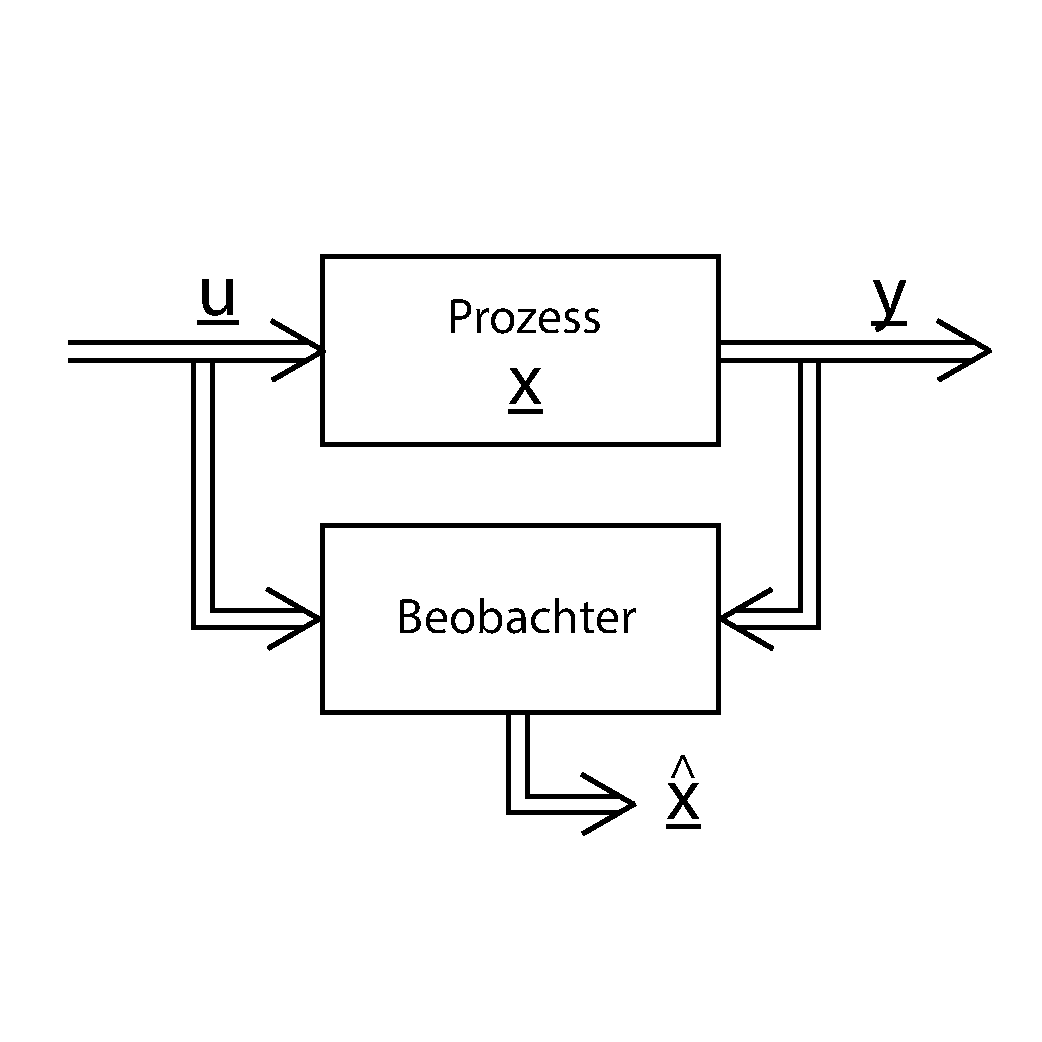
\includegraphics[width=0.5\textwidth]{Bilder/Beobachter/System_Beobachter.pdf}}
    \caption[System mit Beobachter]{Schematische Darstellung eines allgemeinen Systems mit Beobachter im Zustandsraum}
    \label{fig:Bild44}
\end{figure}

\subsection{Überprüfung der Beobachtbarkeit}

Naheliegend ist zunächst die Überlegung anzustellen, wann sich der Gesamtzustand $\underline{x}$ aus dem Ausgang $\underline{y}$ rekonstruieren lässt. Dies wird auch \textbf{Beobachtbarkeit} des Systems genannt. Konkret gilt der Satz: \\
\newline
\textit{Ein System ist beobachtbar, falls mit der Messung von $\underline{u}$ und $\underline{y}$ nach endlicher Zeit $t$ der unbekannte Zustandsvektor $\underline{x}$ vom System rekonstruiert werden kann.} \\
\newline
Der Beobachter lässt sich auf die Klasse der linearen zeitinvarianten Systeme (LTI) anwenden:

\begin{align}
    \underline{\dot{\hat{x}}} = A \cdot \underline{\hat{x}} + B \cdot \underline{u} + L \left( \underline{y} - C \cdot \underline{\hat{x}}\right)
\end{align}

Ein System ist vollständig beobachtbar, falls für die Beobachtbarkeitsmatrix

\begin{align}
    Q_{\mathrm{Obs}} =
    \begin{pmatrix}
        C \\
        C \cdot A \\
        \vdots \\
        C \cdot A^{n - 1}
    \end{pmatrix}
\end{align}

mit $n\in\mathbb{N}$, $p\in\mathbb{N}$, $A\in\mathbb{R}^{(n\times n)}$, $C\in\mathbb{R}^{(p\times n)}$ für SISO Systeme

\begin{align}
    det(Q_{\mathrm{Obs}}) \neq 0
\end{align}

und für MIMO \bzw SIMO Systeme

\begin{align}
    rank(Q_{\mathrm{Obs}}) = n \quad \text{\bzw} \quad m
\end{align}

gilt, wobei $n$ die Anzahl der linear unabhängigen Zeilen einer Matrix ist und $m$ die Anzahl der linear unabhängigen Spalten. Falls

\begin{align*}
    n &> m: \\
    rank(X) &= m
\end{align*}

und falls

\begin{align*}
    m &> n: \\
    rank(X) &= n.
\end{align*}

Die konkrete C-Matrix für das inverse Pendel

\begin{align}
    C_{\mathrm{Obs}} = 
    \begin{bmatrix}
        1 & 0 & 0 & 0 \\
        0 & 0 & 1 & 0 \\
        0 & 0 & 0 & 1
    \end{bmatrix}
\end{align}

besitzt p Zeilen, wobei sich die Anzahl der Zeilen nach den messbaren Zuständen richtet. Zu erkennen ist, dass bei der Betrachtung nicht wie beim Zustandsreglerentwurf ein SISO System angenommen werden kann, sondern ein SIMO System auf Beobachtbarkeit untersucht wird. Somit muss der Rang der Beobachtbarkeitsmatrix bestimmt werden.\\
Das Aufstellen der Beobachtbarkeitsmatrix führt zu

\begin{align}
    Q_{\mathrm{Obs}} = 
    \begin{bmatrix}
        1 & 0 & 0 & 0 \\
        0 & 0 & 1 & 0 \\
        0 & 0 & 0 & 1 \\
        0 & 1 & 0 & 0 \\
        0 & 0 & 0 & 1 \\
        -0.8502 & 0.0008 & 0 & -2.3333 \\
       26.6505 & -0.0248 & 0 & 5.8333 \\
       -0.8502 & 0.0008 & 0 & -2.3333 \\
        2.0049 & -0.8521 & 0 & 5.4491 \\
       -5.6209 & 26.6557 & 0 & -13.7559 \\
        2.0049 & -0.8521 & 0 & 5.4491 \\
      -27.3408 & 2.0304 & 0 & -17.6849
    \end{bmatrix}.
\end{align}

Der Rang folgt zu:

\begin{align}
    rank(Q_{\mathrm{Obs}}) = 4
\end{align}

Da $m > n$ muss $n = 4$ gelten. Da dies der Fall ist, ist das System beobachtbar.

\subsection{Beobachterentwurf}

\begin{figure}[H]
    \centering
    \fbox{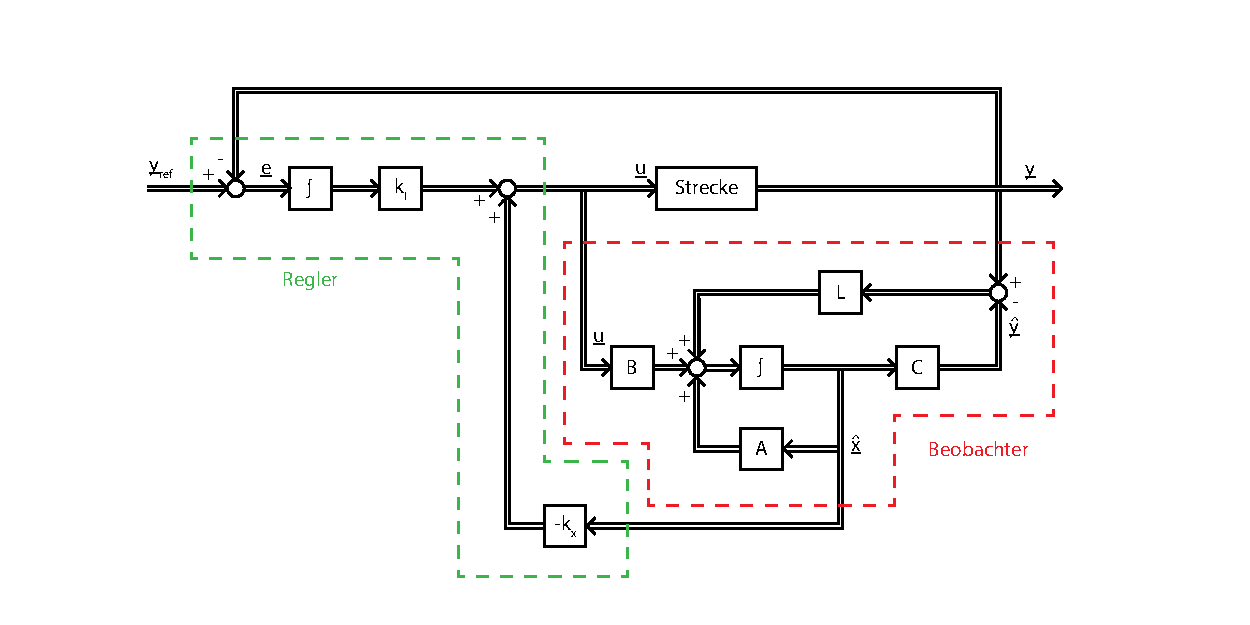
\includegraphics[width=1.0\textwidth]{Bilder/Beobachter/Beobachter_Regler_Strecke.pdf}}
    \caption[Reglerstruktur mit Beobachter]{Schematische Darstellung des Zustandsreglers mit I-Regelung und Beobachter}
    \label{fig:Bild45}
\end{figure}

\subsection{Beobachtervalidierung}